% =====================================================================
%  TA-IND-01 — Informe Académico Individual
%  Análisis crítico comparativo: HDFS frente a Ceph
%  Aplicaciones Distribuidas — UTEQ — 7mo nivel, paralelo B
%
%  ESTADO (14-nov-2026)
%  Aquí va solo lo que se sostiene con trabajo propio: el experimento,
%  sus mediciones, el entorno del estudiante y los anexos. Lo que exige
%  respaldo bibliográfico está marcado con la caja \pendiente y se
%  redactará a medida que se verifique cada artículo del corpus.
%
%  Compilación:  pdflatex main.tex → biber main → pdflatex ×2
% =====================================================================
\documentclass[12pt,a4paper]{article}

\usepackage[utf8]{inputenc}
\usepackage[T1]{fontenc}
\usepackage[english,spanish,es-tabla]{babel}
% autostyle=true hace que las comillas sigan al idioma activo: así la
% bibliografía usa comillas inglesas de IEEE y el texto sigue en español.
\usepackage[autostyle=true]{csquotes}
\usepackage{amsmath}

\usepackage[top=2.6cm,bottom=2.6cm,left=2.5cm,right=2.5cm]{geometry}
\usepackage{lmodern}
\usepackage{microtype}
\usepackage{parskip}
\usepackage{xcolor}

\usepackage{graphicx}
\usepackage{booktabs}
\usepackage{array}
\usepackage{caption}
\captionsetup{font=small,labelfont=bf,justification=justified}
\usepackage{float}

% Se usa para el marco de la carátula.
\usepackage{tikz}
\usetikzlibrary{calc}

% Bibliografía en IEEE. language=english evita que babel-spanish traduzca
% las abreviaturas (y, n.o, págs.) y las comillas, que no son IEEE.
\usepackage[style=ieee,backend=biber,sorting=none,language=english]{biblatex}
\addbibresource{../referencias.bib}

\usepackage[hidelinks]{hyperref}
\usepackage{url}

\usepackage{fancyhdr}
\setlength{\headheight}{15pt}
\pagestyle{fancy}
\fancyhf{}
\fancyhead[L]{\small Aplicaciones Distribuidas}
\fancyhead[R]{\small TA-IND-01}
\fancyfoot[C]{\thepage}
\renewcommand{\headrulewidth}{0.4pt}

% Caja para lo que todavía no tiene respaldo documental.
\newcommand{\pendiente}[1]{%
  \par\medskip
  \noindent\colorbox{gray!10}{%
    \parbox{\dimexpr\linewidth-2\fboxsep}{%
      \small\textbf{Pendiente.} #1}}%
  \par\medskip}

\newif\ifhayfuentes
\hayfuentestrue   % la bibliografía se imprime cuando existan citas verificadas

\graphicspath{{../capturas/}{../figs/}{./}}

\begin{document}

% =====================================================================
%  CARÁTULA
% =====================================================================
\definecolor{verdeuteq}{HTML}{7CBA42}

% Campo de la carátula: etiqueta en negrita y valor debajo.
\newcommand{\campoc}[2]{%
  \vspace{0.28cm}%
  {\bfseries #1\par}%
  \vspace{0.05cm}%
  {#2\par}}

\begin{titlepage}
\thispagestyle{empty}
\centering
\fontfamily{ptm}\selectfont

% Marco verde en L y línea negra, según el modelo de la asignatura.
\begin{tikzpicture}[remember picture, overlay]
  \fill[verdeuteq] ([xshift=1.50cm,yshift=-1.11cm]current page.north west)
        rectangle ([xshift=19.48cm,yshift=-1.55cm]current page.north west);
  \fill[verdeuteq] ([xshift=1.50cm,yshift=-1.11cm]current page.north west)
        rectangle ([xshift=1.94cm,yshift=-28.20cm]current page.north west);
  \draw[black, line width=0.7pt]
        ([xshift=1.50cm,yshift=-1.11cm]current page.north west)
        rectangle ([xshift=19.58cm,yshift=-28.33cm]current page.north west);
\end{tikzpicture}

\vspace*{1.0cm}


\includegraphics[height=1.9cm]{logo-uteq.png}\hspace{1.9cm}%

\includegraphics[height=1.9cm]{logo-facultad.png}

\vspace{0.45cm}
{\Large\bfseries UNIVERSIDAD TÉCNICA ESTATAL DE QUEVEDO\par}
\vspace{0.24cm}
{\bfseries FACULTAD DE CIENCIAS DE LA COMPUTACIÓN Y DISEÑO DIGITAL\par}

\campoc{CARRERA:}{INGENIERÍA EN SOFTWARE 7MO NIVEL}
\campoc{ASIGNATURA:}{APLICACIONES DISTRIBUIDAS}
\campoc{DOCENTE:}{ING. GLEISTON CICERÓN GUERRERO ULLOA}
\campoc{TEMA:}{TA-IND-01 — ANÁLISIS CRÍTICO COMPARATIVO DE UN SISTEMA\\DISTRIBUIDO REAL: HDFS FRENTE A CEPH}
\campoc{ESTUDIANTE:}{MENDOZA BERMELLO ANGELLO AGUSTÍN}
\campoc{PARALELO:}{B}
\campoc{FECHA:}{15 DE NOVIEMBRE DE 2026}
\campoc{REPOSITORIO:}{\small\url{https://github.com/Amendozab5/ta-ind-01-HDFS-Ceph}}

\vspace{0.5cm}
{\bfseries AÑO LECTIVO 2026 — 2027\par}
\vspace{0.08cm}
{\itshape Quevedo — Los Ríos — Ecuador\par}

\end{titlepage}

% =====================================================================
%  RESUMEN
% =====================================================================
\section*{Resumen}
\addcontentsline{toc}{section}{Resumen}

Este informe analiza HDFS y lo compara con Ceph, dos sistemas que resuelven el mismo problema, guardar datos replicados sobre servidores comerciales, con decisiones opuestas sobre dónde reside la ubicación de los datos. El análisis aplica las transparencias de distribución, el teorema CAP con su extensión PACELC, los modelos de comunicación y la tolerancia a fallos, y se apoya en un experimento propio. Se montó un clúster de cuatro contenedores, un NameNode y tres DataNodes con replicación tres; se subió un archivo de 1386 bytes, se comprobó con \texttt{fsck} que tenía tres copias y se apagó un nodo. El NameNode tardó veinte minutos en declararlo muerto, el doble de lo que arroja el cálculo teórico. En ese lapso el archivo apareció como sano y a la vez como falto de una réplica, y al reiniciar el nodo recuperó sus tres copias sin intervención. Se concluye que el tiempo de detección es un umbral y no un tiempo de reacción, que el indicador que delata la degradación es el número de bloques bajo replicación, y que HDFS custodia la ubicación en un servidor que no se escala mientras Ceph la calcula en el cliente.

\newpage

% =====================================================================
%  1. INTRODUCCIÓN
% =====================================================================
\section{Introducción}

La elección de HDFS responde a una razón práctica: permite levantar un clúster real en un portátil. Con cuatro contenedores se tiene un NameNode y tres DataNodes funcionando, así que es posible ver qué pasa cuando un nodo se cae en lugar de imaginarlo.

La industria de TI y las organizaciones generan hoy unos 2,5 exabytes de datos, y HDFS es uno de los marcos más usados para procesarlos \cite[p.~2830]{dhulavvagol2023performance}. Para no perder información cuando un equipo falla, el sistema guarda copias en nodos distintos, y esas copias consumen espacio y recursos \cite[p.~18551]{ahmed2023replication}. Cuando la escala crece, ese gasto de espacio pasa a ser el problema, y por eso HDFS empezó a ofrecer codificación de borrado como alternativa a la copia completa \cite[p.~3]{kim2021erasure}.

El problema de fondo está descrito en la literatura. El teorema CAP, en la formulación de Brewer, dice que cuando la red se parte un sistema distribuido tiene que renunciar a la consistencia o a la disponibilidad \cite[p.~1]{lee2023consistency}. Consistencia quiere decir que todos los componentes coinciden en el valor de un dato compartido; disponibilidad, que el sistema puede atender las peticiones que leen o modifican ese dato.

La técnica con la que los sistemas repartidos compran disponibilidad es la replicación. La revisión de Jaafar Ahmed y sus coautores la presenta como la forma de crecer en escala y señala que su aporte principal es la disponibilidad y el rendimiento: si un nodo falla, el sistema sigue trabajando porque quedan los demás \cite[p.~172]{ahmed2023consistency}. Esa frase describe lo que pasó cuando se apagó \texttt{dn2}.

Lo que la literatura no resuelve por adelantado es qué lado del compromiso conviene en cada caso. Lee concluye que la elección depende de la aplicación, y que hay aplicaciones donde se sacrifica la consistencia y otras donde se sacrifica la disponibilidad \cite[p.~10]{lee2023consistency}. Eso deja abierta la pregunta que interesa aquí: qué hace un sistema concreto cuando le falta un nodo.

El experimento responde una pregunta concreta. Si hay tres copias de cada bloque y se cae un nodo, ¿qué informa el sistema, cuánto tarda en informarlo y qué pasa con el archivo mientras tanto? Se contesta con comandos y capturas, y el resultado no depende de una opinión.

% =====================================================================
%  2. ARQUITECTURA
% =====================================================================
\section{Arquitectura del sistema}

La figura~\ref{fig:arq} es el esquema elaborado antes de empezar a experimentar. A la izquierda está HDFS con el clúster montado, y el nodo que se apagó va en rojo. A la derecha está Ceph, que resuelve el mismo problema con otra idea: no tener un servidor que guarde dónde quedó cada dato.

\begin{figure}[H]
\centering
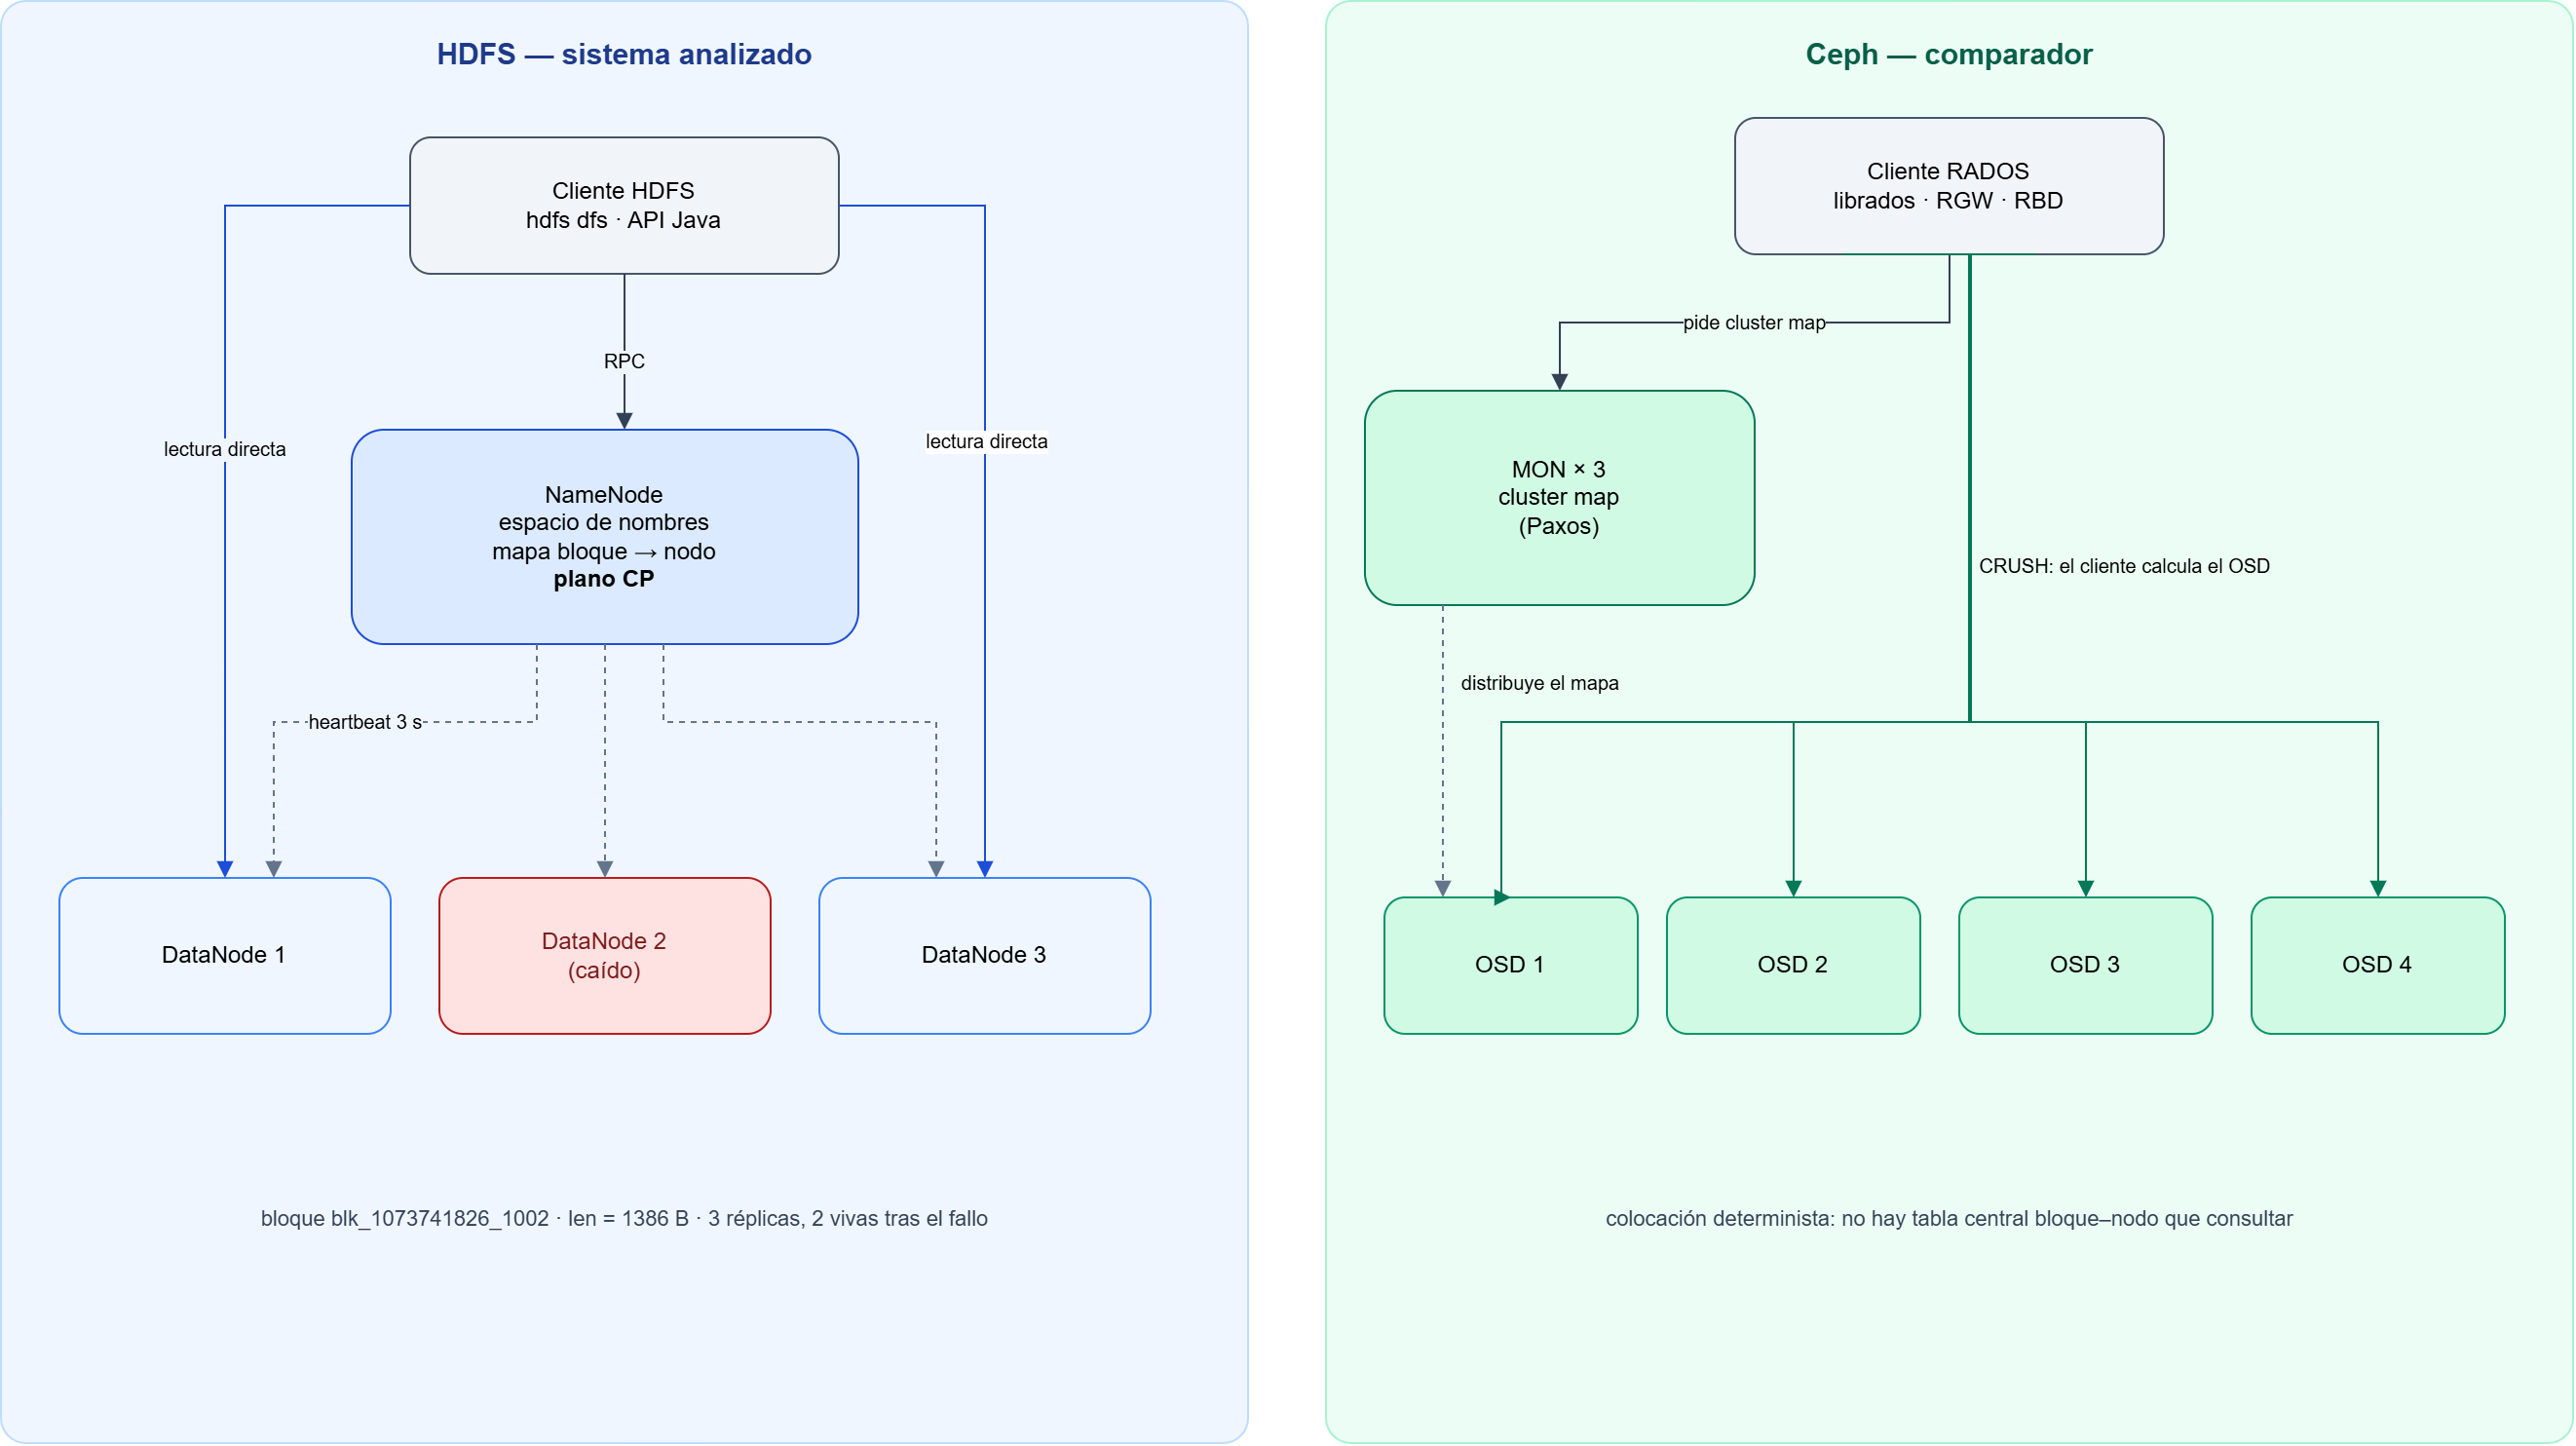
\includegraphics[width=\textwidth]{arquitectura-hdfs-ceph.png}
\caption[Esquema de los dos sistemas]{Esquema hecho para este informe. A la izquierda, HDFS con el NameNode como plano de control y los tres DataNodes del clúster; el nodo apagado va en rojo. A la derecha, Ceph, con los monitores y la colocación por CRUSH.}
\label{fig:arq}
\end{figure}

En HDFS el cliente pide al NameNode la información de dónde están los datos y después trabaja directamente con los DataNodes \cite[p.~4]{kim2021erasure}. El NameNode es, entonces, quien administra los metadatos, y ahí está el límite: se pueden añadir DataNodes, pero no NameNodes, porque la arquitectura de Hadoop no escala los metadatos, y a la escala de datos actual esa concentración se vuelve un cuello de botella \cite[p.~2830]{dhulavvagol2023performance}.

Ceph evita ese nodo central. Su almacén de objetos se apoya en muchos dispositivos (OSD) y unos pocos monitores que se encargan de gestionarlos; cuando el cliente escribe, los datos se cortan en objetos de tamaño fijo, se agrupan en \emph{placement groups} y cada grupo se mapea a un conjunto de OSD mediante CRUSH \cite[p.~1128]{li2023ceph}. El grupo existe precisamente para no tener que seguir cada objeto: un clúster maneja decenas de millones, y Ceph usa el \emph{placement group} como unidad básica de mapeo y replicación \cite[p.~4]{chum2021supporting}. Comparo con Ceph y no con otro sistema de archivos porque resuelve el mismo problema, guardar datos replicados sobre servidores comerciales, tomando la decisión contraria.

% =====================================================================
%  3. ANÁLISIS CON LOS CONCEPTOS DE LA UNIDAD 1
% =====================================================================
\section{Análisis con los conceptos de la Unidad 1}

\subsection{Transparencias de distribución}

Para ordenar el análisis uso las ocho transparencias del modelo ANSA: acceso, ubicación, migración, reubicación, replicación, concurrencia, fallos y persistencia. Las definiciones son del modelo; lo que las fuentes describen es el mecanismo, y de ahí sale si el sistema cumple o no.

En HDFS el cliente obtiene del NameNode la ubicación del archivo y después trabaja con los DataNodes \cite[p.~4]{kim2021erasure}. Ese reparto hace que no necesite conocer la máquina concreta, así que cumple la transparencia de ubicación. En Ceph el cliente deduce el OSD con CRUSH a partir del identificador del grupo y del mapa del clúster \cite[p.~1128]{li2023ceph}, y el mismo almacén se ofrece como objeto, como bloque y como archivo \cite[p.~3]{chum2021supporting}, lo que da transparencia de acceso.

La replicación se cumple en los dos: el cliente escribe una vez y el sistema guarda copias en nodos distintos para dar disponibilidad y fiabilidad \cite[p.~18551]{ahmed2023replication}. De la transparencia de fallos hay evidencia del experimento: con un DataNode caído el archivo se siguió leyendo porque quedaban dos copias. La revisión de Jaafar Ahmed describe el mismo efecto para la replicación en general, porque si un nodo falla el sistema sigue trabajando con los que quedan \cite[p.~172]{ahmed2023consistency}. La persistencia se ve en el montaje: cada contenedor tiene su propio volumen y los bloques sobreviven al reinicio del proceso que los escribió.

Sobre migración, reubicación y concurrencia no es posible pronunciarse. El experimento usó un solo cliente, no movió datos entre nodos mientras estaban en uso, y las fuentes consultadas no describen esos comportamientos para ninguno de los dos sistemas.

\subsection{CAP y PACELC}

El teorema CAP sostiene que un sistema replicado no puede garantizar a la vez consistencia, disponibilidad y tolerancia a particiones, y que ante una partición hay que ceder una de las dos primeras \cite[p.~1]{anagnostakis2025new}. La revisión de Jaafar Ahmed lo plantea en términos de operación: si una réplica no responde dentro del tiempo de espera, el sistema tiene que elegir entre devolver un dato posiblemente desactualizado o declararse no disponible \cite[p.~172]{ahmed2023consistency}.

PACELC extiende la pregunta al caso en que no hay partición. Si la hay, se elige entre disponibilidad y consistencia; si no la hay, el compromiso es entre latencia y consistencia, porque sostener la consistencia obliga a coordinar las réplicas y esa coordinación tarda \cite[p.~172]{ahmed2023consistency}. De ahí salen cuatro clases, y el mismo artículo pone a HBase y BigTable entre las PC/EC y a Cassandra y Dynamo entre las PA/EL.

Ninguna de las fuentes clasifica a HDFS, así que lo que sigue es una lectura del mecanismo ya descrito. En el plano de metadatos el sistema concentra la decisión en el NameNode, que no se escala \cite[p.~2830]{dhulavvagol2023performance}: sin ese nodo no hay manera de saber dónde están los bloques, de modo que el sistema no puede seguir respondiendo. Eso lo ubica del lado de la consistencia en ese plano. En el plano de datos ocurrió lo contrario: con un DataNode apagado el archivo se siguió leyendo y el \texttt{fsck} no reportó corrupción. La caída de un nodo no produjo el dilema que describe el teorema, así que ese resultado no sirve para clasificar al sistema en CAP; para eso haría falta una partición de red real, que no se provocó.

Para Ceph el corpus tampoco da una clasificación. Lo único anotable es que su colocación se calcula sin consultar a un servidor \cite[p.~1128]{li2023ceph}, lo que en PACELC apuntaría al lado de la latencia, aunque sin evidencia directa.

\subsection{Modelos de comunicación}

En HDFS la comunicación está partida en dos canales. El cliente pide los metadatos al NameNode mediante RPC, un protocolo montado sobre sockets y más lento que ellos, y para leer o escribir el contenido usa sockets directamente contra los DataNodes \cite[p.~11]{tchaye2019hpf}. El esquema es cliente-servidor, y la separación importa porque el canal de control mueve unas pocas peticiones mientras que el de datos mueve el volumen \cite[p.~4]{kim2021erasure}.

En Ceph el cliente también es cliente-servidor, pero no consulta una tabla: calcula el OSD a partir del identificador del grupo y del mapa del clúster \cite[p.~1128]{li2023ceph}. Eso le ahorra una consulta por operación, a cambio de que el cálculo lo haga el propio cliente. Ninguno de los dos sistemas se describe en las fuentes como mensajería con colas; lo que aparece son llamadas y flujos punto a punto. El costo de coordinación surge cuando se exige consistencia, porque entonces hay que sincronizar a las réplicas y ese intercambio añade latencia \cite[p.~1]{ahmed2023consistency}.

\subsection{Tolerancia a fallos}

Los fallos que enfrentan estos sistemas no son solo discos estropeados: también caídas del sistema de archivos, errores de operación y desastres, y cualquiera de ellos puede sacar un nodo de servicio y costar datos \cite[p.~1]{lei2024fpga}. Las dos técnicas para cubrirlos son la redundancia por réplicas y la codificación de borrado \cite[p.~1]{lei2024fpga}, y en HDFS la primera es la vía por defecto: cada bloque se guarda en tres DataNodes para no perderlo si uno falla \cite[p.~1]{tchaye2019hpf}.

Detectar el fallo depende de un tiempo de espera, que la revisión de Jaafar Ahmed identifica como el mecanismo principal de detección en sistemas distribuidos y que obliga a elegir entre dos males: si es corto, el sistema declara particiones que no existen; si es largo, tarda en reaccionar \cite[p.~172]{ahmed2023consistency}. La recuperación tiene un costo simétrico, porque con codificación de borrado hay que decodificar, y eso pesa sobre todo en datos de acceso frecuente \cite[p.~1]{lei2024recovery}.

El mecanismo de la codificación es aritmético: si se pierden hasta $m$ bloques de datos o de paridad, la decodificación necesita al menos $k$ para reconstruir lo que falta \cite[p.~3]{lei2024recovery}. La replicación no calcula nada, porque la copia ya existe; lo que se ajusta es cuántas copias mantener, y esa política puede variar según el uso del archivo \cite[p.~18551]{ahmed2023replication}. En el experimento se vio la versión simple de ese proceso: el bloque volvió a tres copias en unos tres minutos sin que se emitiera ninguna orden. No se encontró un informe público de un incidente real de HDFS que pudiera citarse, así que el caso documentado es el de este trabajo.

% =====================================================================
%  4. EXPERIMENTACIÓN PROPIA
% =====================================================================
\section{Experimentación propia}

\subsection{Montaje}

Se usó Docker Compose sobre Windows 11 con contenedores Linux, y las imágenes \texttt{bde2020} de Hadoop 3.2.1. La red fue una puente aislada, con un volumen propio por contenedor para que los datos sobrevivan a un reinicio. El NameNode quedó en \texttt{172.18.0.4} y los DataNodes en \texttt{172.18.0.3}, \texttt{172.18.0.2} y \texttt{172.18.0.5}.

El archivo de prueba es un manifiesto de 1386 bytes con el equipo, la topología y los pasos. Su tamaño da igual: la replicación trabaja sobre bloques, no sobre archivos enteros, y el \texttt{fsck} lo reporta como un solo bloque de 1386 bytes.

La secuencia fue: levantar el clúster, subir el archivo a \texttt{/uteq/aamen/datos.txt}, verificar las tres réplicas, apagar \texttt{dn2}, esperar, mirar el reporte y el \texttt{fsck}, leer el archivo con un nodo caído y volver a encender \texttt{dn2}.

\begin{figure}[H]
\centering
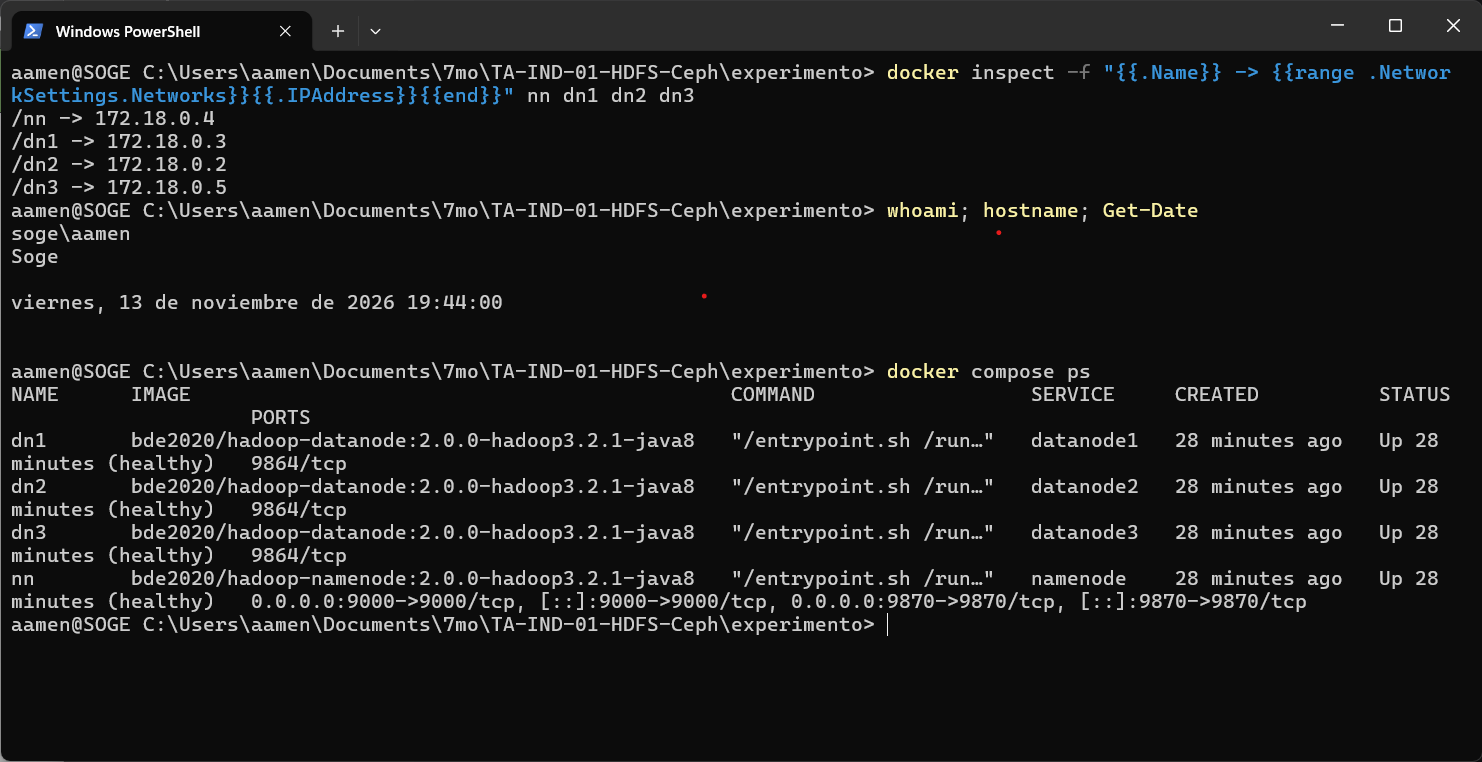
\includegraphics[width=0.95\textwidth]{01-cluster-arriba.png}
\caption{El clúster antes del fallo: los cuatro contenedores arriba y el NameNode respondiendo en el puerto 9870.}
\label{fig:arriba}
\end{figure}

\subsection{Qué se observó}

Se apagó \texttt{dn2} y el sistema no reaccionó enseguida. El último contacto con el nodo fue a las 02:41:39 UTC y la declaración de muerte llegó a las 03:01:47 UTC: veinte minutos. Con los valores de fábrica la cuenta da diez minutos y treinta segundos, así que lo medido es el doble. La explicación que se sostiene es que ese cálculo es un umbral y no un reloj, y que al umbral hay que sumarle la espera hasta la siguiente revisión del NameNode. No se comprobó en el código, así que queda como suposición.

Cuando por fin lo dio por muerto, el reporte mostró dos nodos vivos y uno caído, con un bloque bajo replicación. El \texttt{fsck} del archivo devolvió esto en la misma ejecución:
\begin{quote}\small
\texttt{Status: HEALTHY}\\
\texttt{Under-replicated blocks: 1 (100.0 \%)}\\
\texttt{Average block replication: 2.0}\\
\texttt{Missing replicas: 1 (33.333332 \%)}
\end{quote}
El bloque era \texttt{blk\_1073741826\_1002}, de 1386 bytes, con dos copias en vez de tres. Lo llamativo son las dos primeras líneas juntas: la herramienta dice que el archivo está sano y en la misma salida dice que le falta una réplica. Las dos frases conviven, pero explicar por qué obliga a apoyarse en la documentación, y eso queda pendiente.

El archivo se siguió leyendo sin problema desde las dos copias que quedaban. Aquí conviene aclarar qué evidencia existe: se guardó el reporte y el \texttt{fsck}, no una captura de la lectura. Después se encendió \texttt{dn2} y el \texttt{fsck} volvió a mostrar tres réplicas, \texttt{Live\_repl=3} y cero bloques bajo replicación. Entre la muerte declarada y esa salida pasaron unos tres minutos, que es lo que tardó en reconstruirse la copia que faltaba.

\begin{figure}[H]
\centering
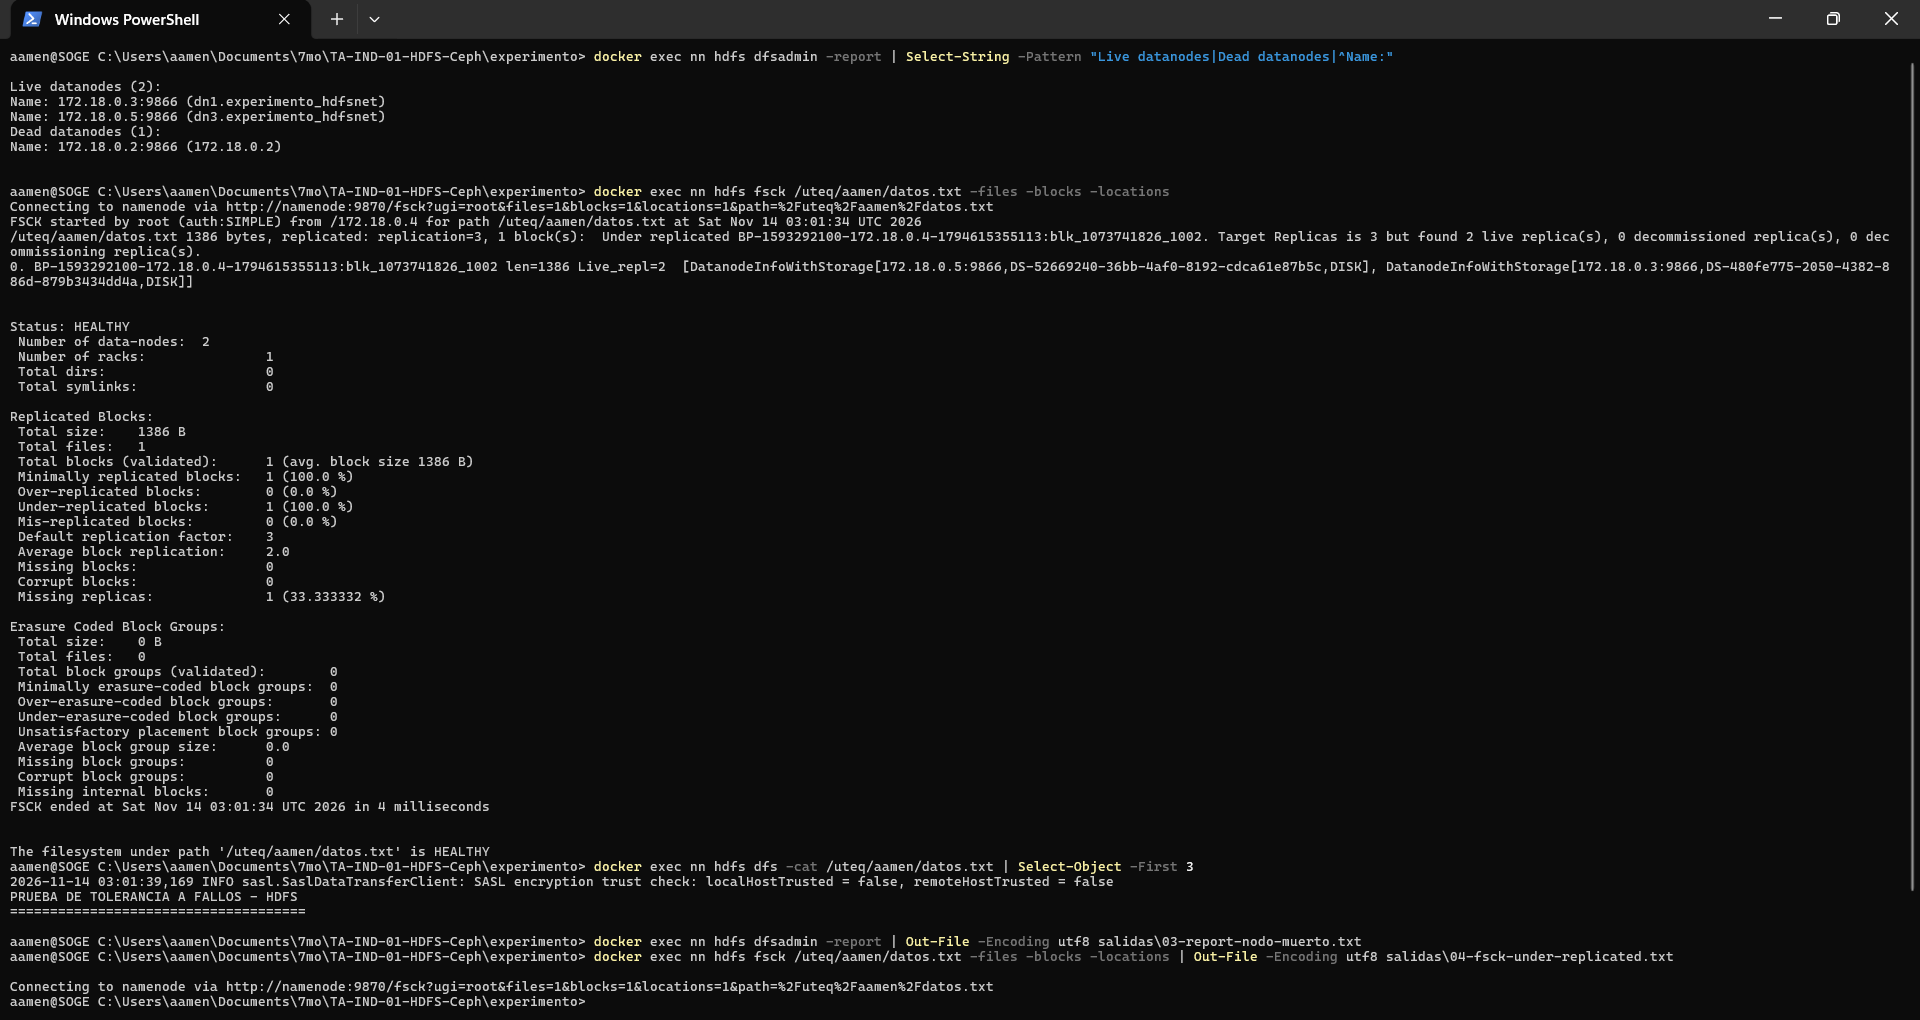
\includegraphics[width=0.95\textwidth]{04-estado-degradado.png}
\caption{Estado degradado: el mismo bloque aparece como \texttt{HEALTHY} y como bajo replicación, con dos copias de tres.}
\label{fig:deg}
\end{figure}

\begin{figure}[H]
\centering
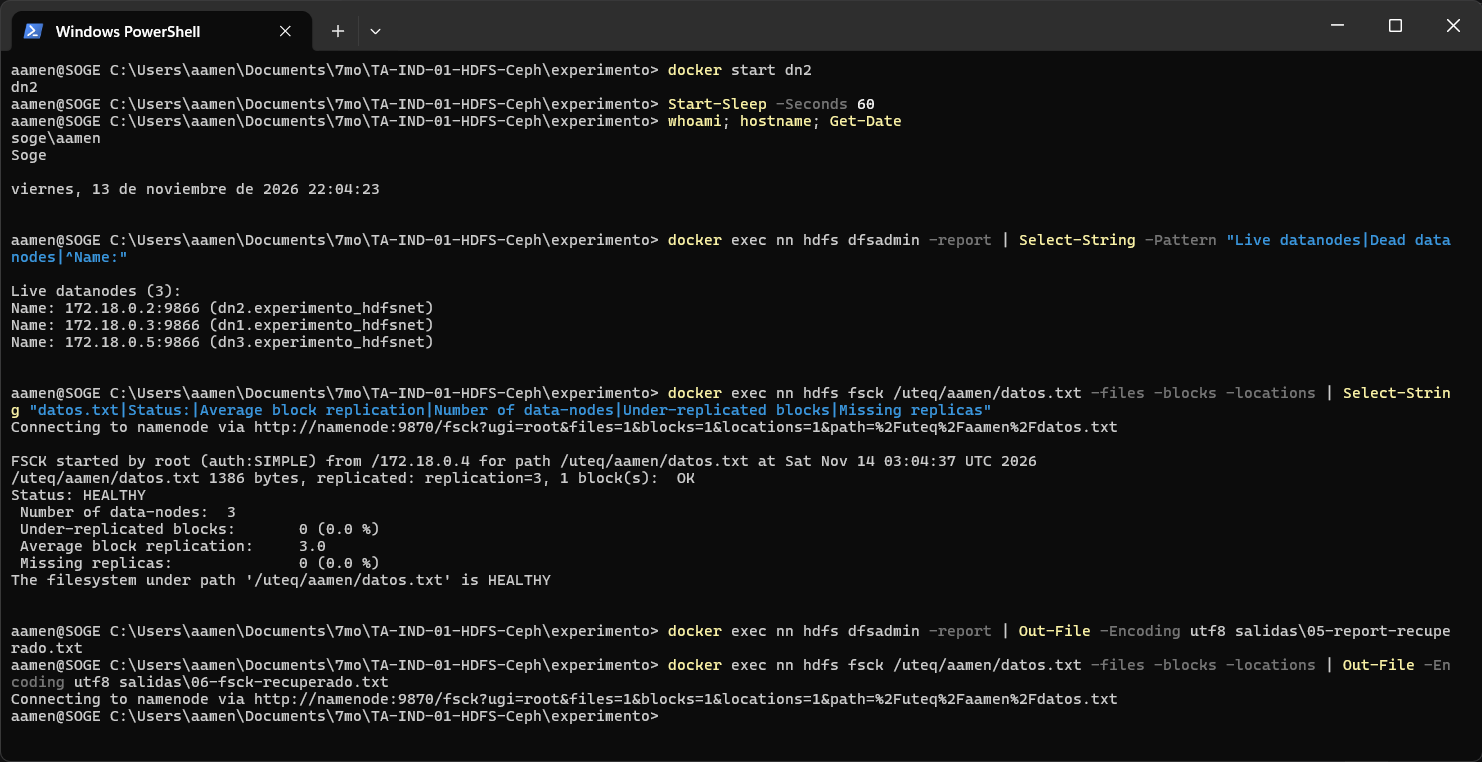
\includegraphics[width=0.95\textwidth]{07-recuperacion.png}
\caption{Después de encender el nodo, el bloque vuelve a tres réplicas sin ninguna orden de reconstrucción.}
\label{fig:rec}
\end{figure}

\subsection{Los tres momentos}

La tabla~\ref{tab:med} junta los valores de las salidas guardadas en \texttt{experimento/salidas/}.

\begin{table}[H]
\centering
\small
\caption{Estado del clúster en los tres momentos del experimento.}
\label{tab:med}
\begin{tabular}{@{}lccc@{}}
\toprule
Indicador & 3 DataNodes & Un nodo caído & Recuperado \\
\midrule
DataNodes vivos              & 3 & 2 & 3 \\
Réplicas del bloque          & 3 & 2 & 3 \\
Under-replicated blocks      & 0 & 1 (100.0 \%) & 0 \\
Missing replicas             & 0 & 1 (33.33 \%) & 0 \\
Average block replication    & 3.0 & 2.0 & 3.0 \\
Estado de \texttt{fsck}      & \texttt{HEALTHY} & \texttt{HEALTHY} & \texttt{HEALTHY} \\
Capacidad configurada        & 2.95 TB & 1.97 TB & 2.95 TB \\
\bottomrule
\end{tabular}
\end{table}

\subsection{Qué se puede afirmar y qué no}

Con estos datos se pueden afirmar tres cosas. Que el tiempo de detección medido duplica el del cálculo, y que por eso ese cálculo no sirve como tiempo de reacción. Que el dato que delata el problema no es el estado general del \texttt{fsck} sino el número de bloques bajo replicación, porque el archivo estuvo marcado como sano con una copia de menos. Y que la vuelta a tres copias no necesitó intervención alguna.

Lo que no se puede afirmar también es importante. Los cuatro contenedores comparten el disco del portátil, así que se probó la tolerancia del protocolo y no la del hardware: si el disco falla, se van las tres copias a la vez. Nunca se apagó el NameNode, así que no se sabe qué pasa cuando falla el plano de control. Y no se probó la codificación de borrado, que era el contraste natural con la replicación.

El resultado que más importa no es el tiempo, sino el par de líneas que el \texttt{fsck} devolvió juntas: \texttt{HEALTHY} y \texttt{UNDER-REPLICATED}. Los dos indicadores responden preguntas distintas. El primero dice si los bloques existen y coinciden sus sumas; el segundo, con cuántas copias se cuenta. HDFS guarda tres copias de cada bloque justamente para no perder el dato si un DataNode falla \cite[p.~1]{tchaye2019hpf}, y los esquemas con redundancia ajustan ese nivel a la cantidad de fallos que quieren tolerar \cite[p.~1]{lei2024recovery}. Con dos copias el archivo no había perdido nada, pero ya no aguantaba un segundo fallo. Marcar \texttt{HEALTHY} no era un error: informaba de integridad, no del margen que quedaba.

Para la clasificación en CAP el experimento sirve a medias. El teorema reparte las garantías entre consistencia, disponibilidad y tolerancia a particiones \cite[p.~1]{anagnostakis2025new}, y lo que se degradó en el clúster no fue ninguna de las tres, sino el margen de copias, que el teorema ni considera. La revisión de Jaafar Ahmed sostiene que el sistema entra en modo partición cuando una réplica no responde dentro del tiempo de espera \cite[p.~172]{ahmed2023consistency}, y bajo esa definición la caída de \texttt{dn2} sí produjo una partición: había que elegir, y el sistema siguió entregando lecturas. Eso describe al plano de datos como favorable a la disponibilidad, pero no alcanza para etiquetar al sistema entero, porque el plano de metadatos nunca se puso a prueba.

% =====================================================================
%  5. EJEMPLOS DEL ENTORNO DEL ESTUDIANTE
% =====================================================================
\section{Ejemplos del entorno del estudiante}

El uso diario incluye varios sistemas repartidos que pasan inadvertidos.

El \textbf{portal de la universidad}. Cuando se sube un trabajo, el archivo se va a un servidor y desaparece del equipo local. Se ve una barra que avanza, y nada más. No se sabe en qué máquina quedó, si hay una copia o tres, ni dónde está esa máquina. Es cómodo, pero no hay forma de saber si la entrega está duplicada.

El \textbf{almacenamiento en la nube}. Sincroniza una carpeta entre el equipo y el servidor. Cuando se edita el mismo archivo desde dos lados, avisa de un conflicto y obliga a elegir. Eso no se probó en el clúster, así que no se sabe cómo respondería HDFS a dos escrituras a la vez: queda como pregunta abierta.

El \textbf{repositorio Git} de este informe. Cada copia del repositorio tiene la historia completa y el servidor es solo un punto de encuentro. Ocurrió algo útil durante el trabajo: se hizo un cambio desde la web y otro en local, y el envío fue rechazado hasta que se juntaron los dos. Es lo que ocurre cuando dos lados aceptan cambios por su cuenta.

El \textbf{equipo de laboratorio}. Los cuatro contenedores del clúster estaban en el mismo disco. Es lo que ya se anotó en la sección anterior, pero visto desde el otro lado: una topología que parece de tres nodos no lo es si se mira el hardware que la sostiene.

% =====================================================================
%  6. ANÁLISIS COMPARATIVO
% =====================================================================
\section{Análisis comparativo}

La tabla~\ref{tab:comp} compara los dos sistemas con cinco criterios de la Unidad 1. Cada celda se apoya en una de las fuentes revisadas.

\begin{table}[H]
\centering
\small
\caption{Comparación entre HDFS y Ceph en cinco criterios de la Unidad 1.}
\label{tab:comp}
\begin{tabular}{@{}>{\raggedright\arraybackslash}p{3.5cm}>{\raggedright\arraybackslash}p{5.5cm}>{\raggedright\arraybackslash}p{5.5cm}@{}}
\toprule
Criterio & HDFS & Ceph \\
\midrule
Ubicación de los datos &
La guarda el NameNode y el cliente la consulta antes de leer \cite[p.~2830]{dhulavvagol2023performance}. &
Se calcula con CRUSH a partir del identificador del grupo y del mapa del clúster \cite[p.~1128]{li2023ceph}. \\
\addlinespace
Escalabilidad de los metadatos &
Se añaden DataNodes, pero no NameNodes: no hay escalado del servidor de metadatos \cite[p.~2830]{dhulavvagol2023performance}. &
El mapeo se hace por grupo y no por objeto, así que no hay que seguirlos uno a uno \cite[p.~4]{chum2021supporting}. \\
\addlinespace
Unidad de almacenamiento &
Bloque de 128 MB, replicado completo \cite[p.~1]{tchaye2019hpf}. &
Objeto de tamaño fijo, agrupado en \emph{placement groups} para el mapeo \cite[p.~1128]{li2023ceph}. \\
\addlinespace
Durabilidad &
Replicación triple por defecto, igual para todo el sistema de archivos \cite[p.~1]{tchaye2019hpf}. &
Replicación o codificación de borrado, elegible por conjunto de almacenamiento \cite[p.~3]{kim2021erasure}. \\
\addlinespace
Comunicación &
RPC sobre sockets para los metadatos y sockets para los datos \cite[p.~11]{tchaye2019hpf}. &
El cliente calcula el destino y escribe en los OSD, con los monitores como referencia \cite[p.~1128]{li2023ceph}. \\
\bottomrule
\end{tabular}
\end{table}

La primera fila explica las demás. En HDFS la ubicación es un dato que alguien calculó y guardó, y por eso hay un servidor que lo custodia y que no se escala \cite[p.~2830]{dhulavvagol2023performance}; el cliente lo consulta antes de leer \cite[p.~11]{tchaye2019hpf}. En Ceph la ubicación es una función que el cliente resuelve con CRUSH \cite[p.~1128]{li2023ceph}. De ahí sale la diferencia de escalabilidad: en HDFS el límite es el servidor de metadatos, mientras que en Ceph lo que se administra es el grupo y no el objeto \cite[p.~4]{chum2021supporting}.

La durabilidad también se elige distinto. HDFS trae tres copias por defecto y esa decisión vale para todo el sistema de archivos \cite[p.~1]{tchaye2019hpf}, mientras que Ceph permite replicación o codificación de borrado según el conjunto de almacenamiento \cite[p.~3]{kim2021erasure}, y la codificación reduce el espacio a cambio de más cálculo al recuperar \cite[p.~1]{lei2024recovery}. La revisión de Jaafar Ahmed ya señalaba el costo del otro lado: más réplicas dan disponibilidad y rendimiento, pero encarecen el almacenamiento \cite[p.~173]{ahmed2023consistency}.

La consecuencia práctica es que ninguno es mejor en abstracto. HDFS está pensado para archivos grandes: es eficiente con pocos archivos de mucho tamaño y sufre con muchos pequeños \cite[p.~1]{tchaye2019hpf}. Ceph ofrece la misma capacidad como objeto, como bloque y como archivo \cite[p.~3]{chum2021supporting}, lo que sirve cuando un mismo almacén tiene que atender aplicaciones distintas. Lo que se compra con la sencillez de HDFS es un cuello de botella en los metadatos; lo que se paga en Ceph es un cliente que hace más trabajo.

% =====================================================================
%  7. POSTURA CRÍTICA
% =====================================================================
\section{Postura crítica}
\label{sec:critica}

La fortaleza de HDFS está en la coherencia entre lo que supone y lo que hace. Guarda los metadatos en memoria justamente para que el acceso sea rápido, y con pocos archivos grandes ese diseño rinde \cite[p.~1]{tchaye2019hpf}. No es casualidad que se haya vuelto un marco muy usado para procesar grandes volúmenes de datos \cite[p.~2830]{dhulavvagol2023performance}: está especializado, y cuando la carga se parece a su supuesto, la especialización es una ventaja y no una limitación.

El problema es que el mismo mecanismo que da velocidad fija el techo. Como el NameNode vive en memoria, una gran cantidad de archivos pequeños lo satura \cite[p.~1]{tchaye2019hpf}, y como ese servidor no se reparte entre varios, añadir DataNodes no alivia el problema, porque los metadatos no están ahí \cite[p.~2830]{dhulavvagol2023performance}. La replicación triple tiene un costo por el otro lado: tres copias de todo consumen espacio, y el gasto crece con el volumen almacenado \cite[p.~18551]{ahmed2023replication}.

Por eso hay contextos donde HDFS no sería la mejor opción. Con muchos archivos pequeños el sistema se degrada por el lado de los metadatos \cite[p.~1]{tchaye2019hpf}. Cuando el mismo almacén tiene que servir como objeto, como bloque y como archivo, Ceph ofrece las tres formas sobre una sola capacidad \cite[p.~3]{chum2021supporting}. Y cuando el espacio es el recurso crítico, la codificación de borrado reduce el costo que impone la copia completa, a cambio de más cálculo al recuperar \cite[p.~3]{kim2021erasure}.

Lo más valioso del experimento es que muestra el estado intermedio. Un informe hecho sin ejecutar nada puede describir qué pasa cuando un nodo se cae, pero no puede mostrar la pantalla donde el sistema dice que el archivo está sano y que le falta una réplica. Esa imagen obliga a precisar qué significa cada indicador antes de sacar conclusiones.

Lo que falla es el alcance. Al no apagar el NameNode, el trabajo no dice nada del plano de control, y ese escenario quedó sin cubrir. Tampoco se probó la codificación de borrado, ni un disco roto, ni un corte de red. Son tareas que quedan abiertas y así se dejan, sin convertirlas en conclusiones.

% =====================================================================
%  8. CONCLUSIONES
% =====================================================================
\section{Conclusiones}

\begin{itemize}
\setlength{\itemsep}{0.3em}
\item El tiempo de detección medido, veinte minutos, duplica el del cálculo con valores de fábrica. Ese cálculo es un umbral, no un tiempo de reacción.
\item Un archivo puede figurar como sano y tener una réplica de menos. El número de bloques bajo replicación dice más que el estado general.
\item La replicación se recuperó sola en unos tres minutos cuando se encendió el nodo. No hizo falta ninguna orden.
\item Los cuatro nodos compartían disco. Todo lo anterior habla del protocolo, no del hardware.
\end{itemize}

Del análisis de las secciones anteriores se desprende además que la comparación no tiene un ganador único. HDFS concentra la decisión de ubicación en un servidor que no se escala y paga ese precio con un techo en los metadatos \cite[p.~2830]{dhulavvagol2023performance}; Ceph evita ese servidor a cambio de que el cliente resuelva el cálculo \cite[p.~1128]{li2023ceph}. Ambos usan la redundancia para sobrevivir a fallos, pero la gastan distinto: HDFS fija tres copias por defecto para todo el sistema de archivos \cite[p.~1]{tchaye2019hpf}, mientras que Ceph permite elegir entre replicación y codificación según el conjunto de almacenamiento \cite[p.~3]{kim2021erasure}. Elegir entre los dos es decidir a qué se le da prioridad, no cuál es mejor.

% =====================================================================
%  DECLARACIÓN DE USO DE INTELIGENCIA ARTIFICIAL
% =====================================================================
\section{Declaración de uso de inteligencia artificial}

\textbf{Herramienta.} Asistente de programación DeepSeek Harness, modelo DeepSeek Flash, usado en sesión sobre el equipo local.

\textbf{Para qué.} Preparar el entorno del experimento, revisar la redacción y el formato LaTeX del documento y ordenar el repositorio. También para buscar candidatos de fuentes, aunque ninguna se dará por buena sin comprobar sus datos en Crossref, su acceso abierto y el contenido del PDF.

\textbf{Cómo se verificó.} El experimento se ejecutó en el equipo local, y todas las cifras de la sección 4 salen de las salidas de comandos guardadas en el repositorio, no de texto generado. Los datos del clúster, el identificador del bloque y las capturas son de esa ejecución.

% =====================================================================
%  REFERENCIAS
% =====================================================================
\clearpage
\ifhayfuentes
  % Se cambia a inglés solo mientras se imprime la lista, para que las
  % abreviaturas y las comillas sean las de IEEE y no las de babel-spanish.
  \selectlanguage{english}
  \printbibliography[heading=bibintoc,title={Referencias}]
  \selectlanguage{spanish}
\fi

% =====================================================================
%  ANEXOS
% =====================================================================
\appendix
\renewcommand{\thesection}{Anexo \Alph{section}}
\clearpage

\section{Esquema de arquitectura a mano}

El esquema de la figura~\ref{fig:arq} salió de este boceto. Primero se dibujó solo HDFS, que es el sistema que se analiza. Ceph entró después, cuando se decidió contra qué compararlo, y el nodo caído y los datos del bloque salieron del experimento. La foto de ese primer boceto va aquí como evidencia del proceso.

\begin{center}
\IfFileExists{anexo-a-esquema-mano.jpg}{%
  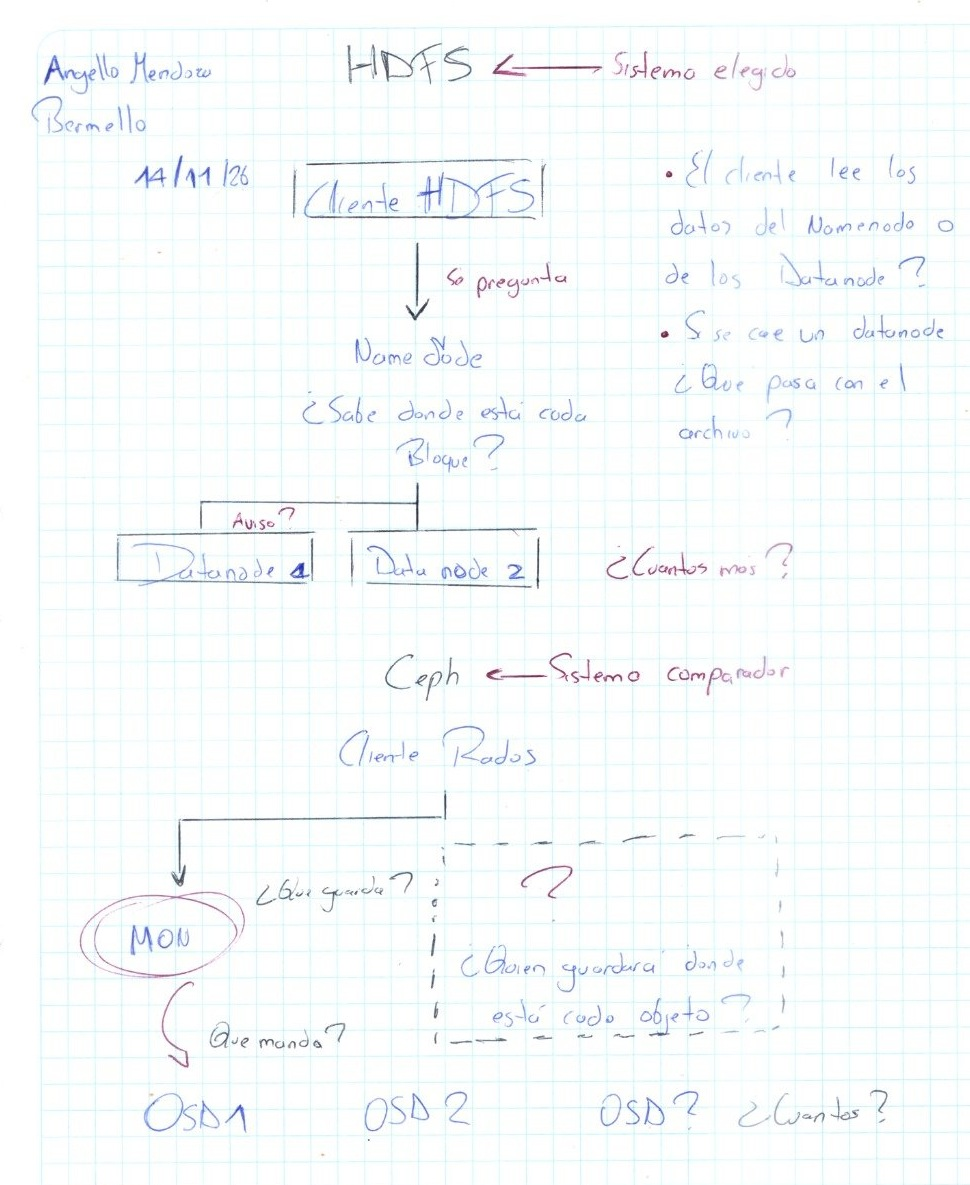
\includegraphics[width=0.92\textwidth,height=0.72\textheight,keepaspectratio]{anexo-a-esquema-mano.jpg}%
}{%
  \fbox{\parbox[c][7cm][c]{0.8\textwidth}{\centering\small
  \textbf{[Pendiente]}\\ Foto del esquema a mano.\\[0.3cm]
  Guardarla como \texttt{informe/anexo-a-esquema-mano.jpg}\\ y aparece sola al compilar.}}%
}
\end{center}

\clearpage
\section{Capturas de lectura de fuentes}

Cada captura corresponde a una cita del texto y muestra la página del artículo donde está el fragmento subrayado.

\noindent\begin{minipage}{\textwidth}
\subsection*{Captura 1. Codificación de borrado frente a replicación}

Kim, \emph{Applied Sciences} 11(8):3298, 2021, página 3. El fragmento subrayado sostiene la afirmación de la introducción sobre que la codificación de borrado reemplaza a la replicación porque gasta menos espacio.

\begin{center}
\IfFileExists{anexo-b-lectura-1.png}{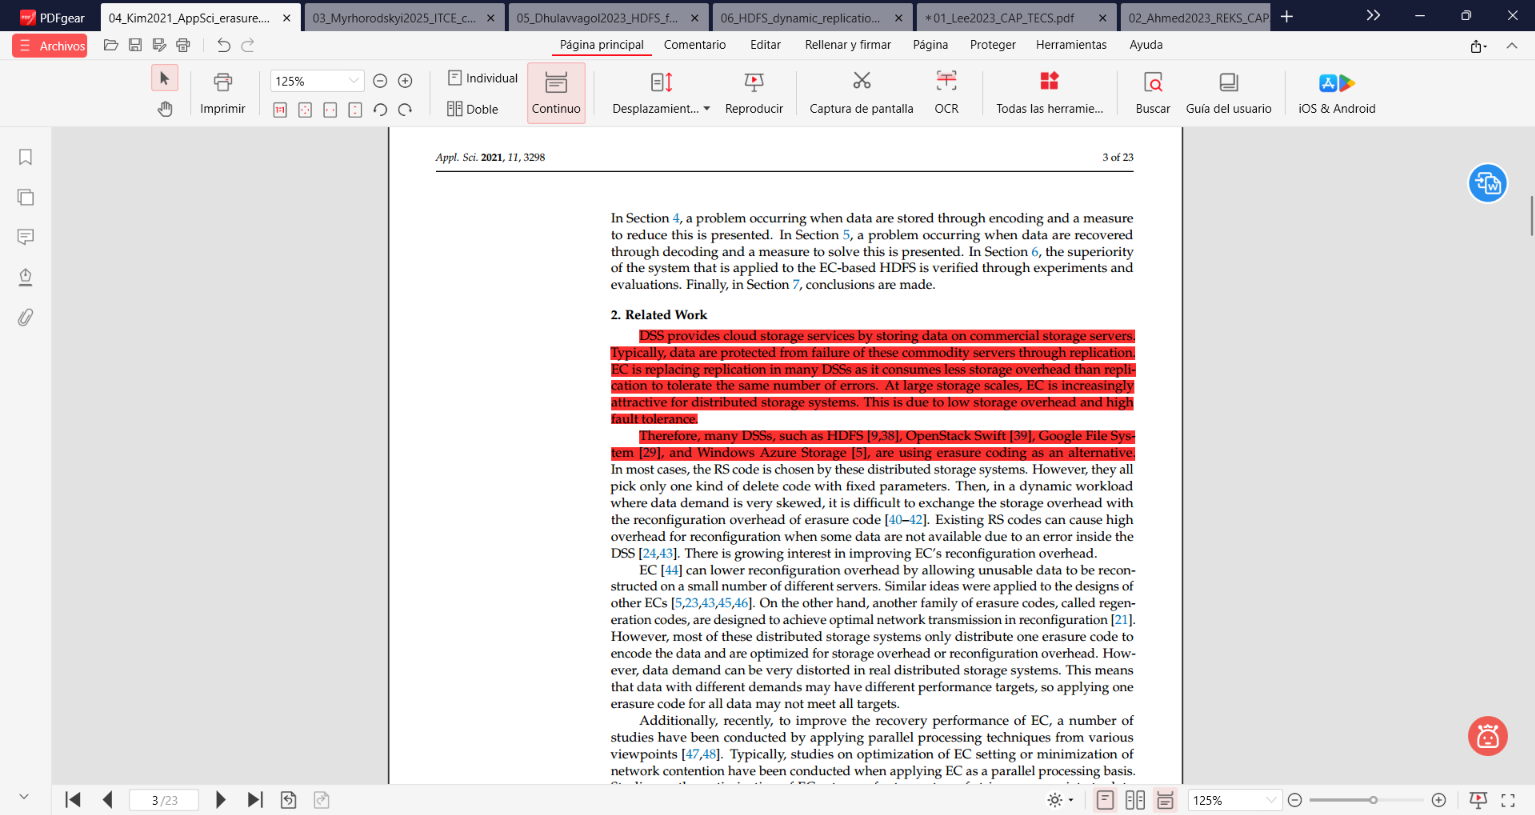
\includegraphics[width=0.95\textwidth]{anexo-b-lectura-1.png}}{%
  \fbox{\parbox[c][5cm][c]{0.8\textwidth}{\centering\small\textbf{[Pendiente]}\\ Fuente 1\\ \texttt{informe/anexo-b-lectura-1.png}}}}
\end{center}
\end{minipage}

\vspace{0.4cm}

\noindent\begin{minipage}{\textwidth}
\subsection*{Captura 2. El costo de replicar de más}

Ahmed y coautores, \emph{Radioelectronic and Computer Systems}, número 2(106), 2023, página 173. Arriba queda el enunciado de PACELC, que está en la página 172 y es el que cito en el análisis; el párrafo subrayado de la página 173 es el que sostiene que más réplicas dan disponibilidad y rendimiento pero encarecen el almacenamiento.

\begin{center}
\IfFileExists{anexo-b-lectura-2.png}{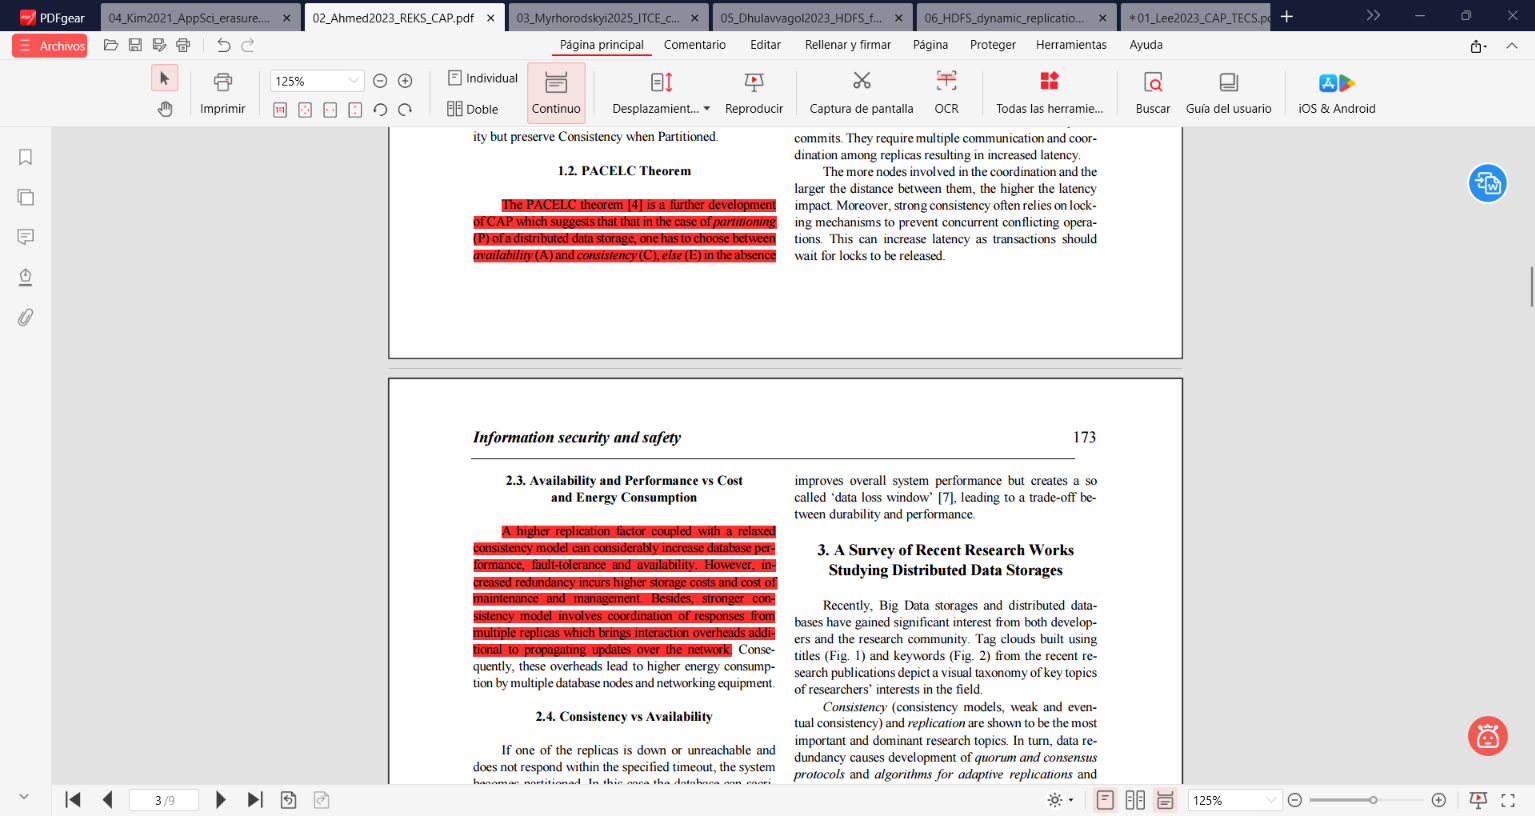
\includegraphics[width=0.95\textwidth]{anexo-b-lectura-2.png}}{%
  \fbox{\parbox[c][5cm][c]{0.8\textwidth}{\centering\small\textbf{[Pendiente]}\\ Fuente 2\\ \texttt{informe/anexo-b-lectura-2.png}}}}
\end{center}
\end{minipage}

\vspace{0.4cm}

\noindent\begin{minipage}{\textwidth}
\subsection*{Captura 3. Las tres interfaces de Ceph}

Chum y coautores, \emph{Electronics} 10(7):847, 2021, página 3. El fragmento subrayado enumera las tres formas en que Ceph ofrece el mismo almacén, objeto, bloque y archivo, que es lo que uso para la transparencia de acceso.

\begin{center}
\IfFileExists{anexo-b-lectura-3.png}{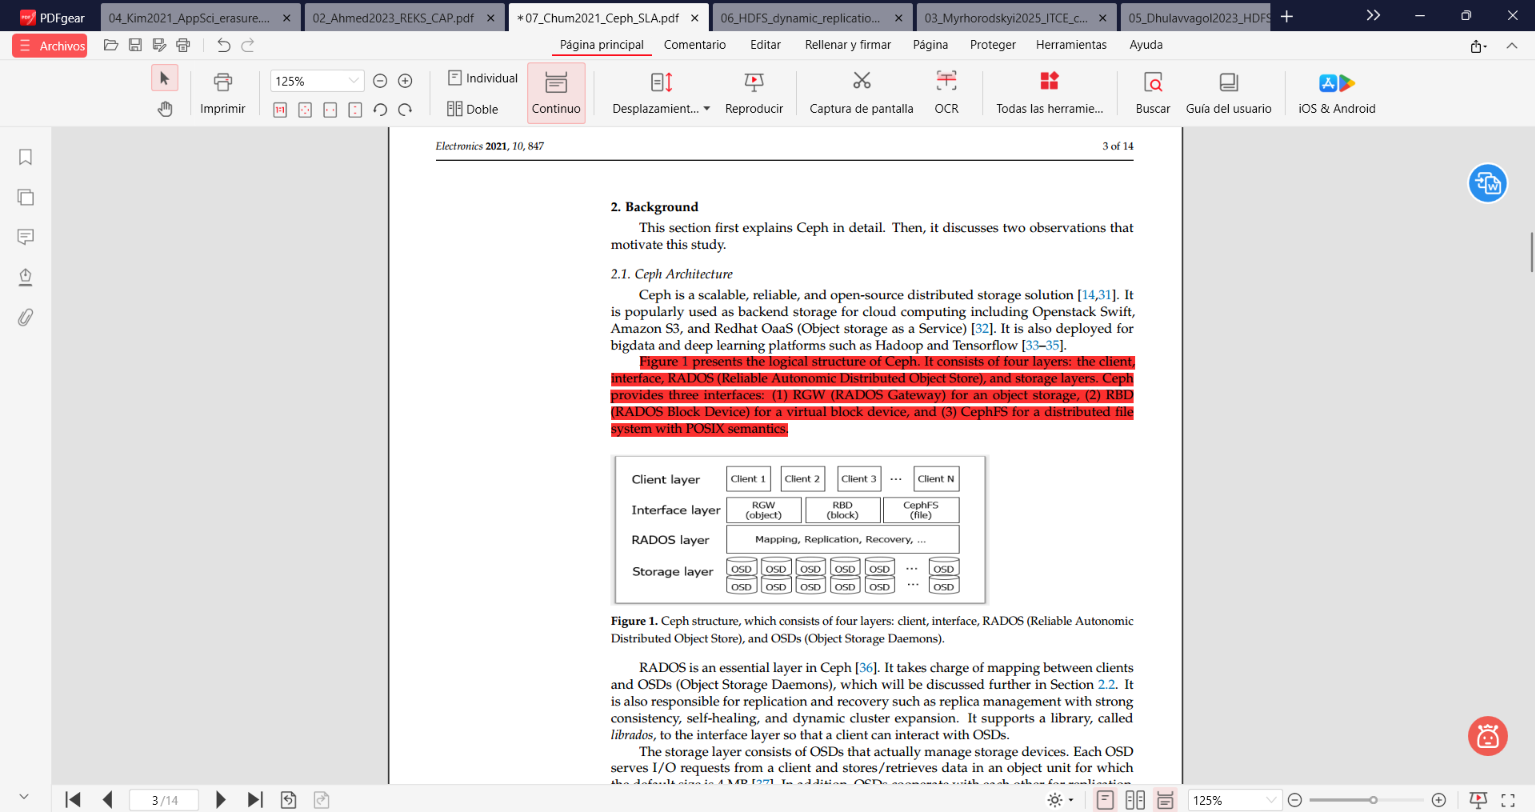
\includegraphics[width=0.95\textwidth]{anexo-b-lectura-3.png}}{%
  \fbox{\parbox[c][5cm][c]{0.8\textwidth}{\centering\small\textbf{[Pendiente]}\\ Fuente 3\\ \texttt{informe/anexo-b-lectura-3.png}}}}
\end{center}
\end{minipage}

\end{document}
